\documentclass[12pt]{article}
\usepackage[margin=1in]{geometry}
\usepackage{graphicx}
\usepackage{tikz}
\usepackage{hyperref}
\usepackage{amsmath}
\usepackage{enumitem}
\usepackage{fancyhdr}
\usepackage{listings}
\usepackage{caption}

\pagestyle{fancy}
\fancyhf{}
\rhead{Spreadsheet Program Report}
\lhead{Your Name}
\rfoot{\thepage}

\title{Spreadsheet Program Report}
\author{Your Name}

\begin{document}
\maketitle

\section{Introduction}
The spreadsheet application supports both simple and advanced formulas. This is implemented through dependencies and dependents for cell structs. The program maintains a separate list of advanced formulas. This report describes the design decisions behind this approach, the program structure, the challenges faced during development, the data structures used for various operations, and how various edge cases are handled.

\section{Design Decisions}
\subsection{Advanced Formulas List}
Instead of storing every cell within a range as a dependency, the program maintains a dedicated list for advanced formulas (defined as a member of the spreadsheet struct). We store only the endpoints of the range and iterate over this global structure to check which ranges include our updated cell. This design has several advantages:
\begin{itemize}[noitemsep]
    \item \textbf{Memory Efficiency:} Large ranges do not lead to a massive dependency list.
    \item \textbf{Performance:} Recalculations are performed by processing only the advanced formulas in the list via topological sorting, thus recalculating a cell at most once.
\end{itemize}

\subsection{Dependency Management}
Simple formulas manage dependencies via AVL trees. Each cell maintains two trees:
\begin{itemize}[noitemsep]
    \item \textbf{Dependencies:} The cells on which the current cell depends.
    \item \textbf{Dependents:} The cells that depend on the current cell.
\end{itemize}
These trees ensure efficient lookup, insertion, and deletion operations.

\subsection{Recalculation Process}
Recalculation is performed in two stages:
\begin{enumerate}[noitemsep]
    \item \textbf{Local Recalculation:} The function \texttt{recalc\_cell()} computes the cell's new value based on its operation (arithmetic or advanced formula).
    \item \textbf{Propagation:} \texttt{recalcUsingTopoOrder()} propagates the change to dependent cells in topologically sorted order. This ensures that each cell is updated only after all its dependencies have been recalculated.
\end{enumerate}

\section{Challenges Faced}
After finalizing the design decisions, several challenges were encountered during implementation:
\begin{enumerate}[noitemsep]
    \item \textbf{Memory Overhead:} The normal approach of storing every cell in the dependency list for range functions consumed a large amount of memory. To address this, we moved to using a dedicated global structure (the advanced formulas list) that stores only the endpoints of the range.
    \item \textbf{Cycle Detection Efficiency:} Implementing cycle detection was challenging because, with the global advanced formulas structure, not all cells were stored as dependencies. The normal DFS approach for checking cycles in long dependency chains proved too slow. We therefore switched to a BFS approach, which was better suited for this design and improved performance significantly.
\end{enumerate}

\section{Data Structures Used for Various Operations}
The efficiency and robustness of our spreadsheet application are driven by carefully selected data structures:
\begin{itemize}[noitemsep]
    \item \textbf{AVL Trees:}
    \begin{itemize}[noitemsep]
        \item Used for managing dependencies and dependents for each cell.
        \item They provide balanced search trees for fast insertions, deletions, and lookups.
    \end{itemize}
    \item \textbf{Linked Lists (Queues):}
    \begin{itemize}[noitemsep]
        \item Employed in the BFS-based cycle detection algorithm.
        \item These queues help traverse the dependency graph efficiently during cycle checks and topological ordering.
    \end{itemize}
    \item \textbf{Arrays:}
    \begin{itemize}[noitemsep]
        \item The advanced formulas list is maintained as a dynamic array, which stores pointers to cells that contain advanced formulas.
        \item This structure provides quick access and iteration when recalculating advanced formulas.
    \end{itemize}
    \item \textbf{Contiguous Memory Blocks:}
    \begin{itemize}[noitemsep]
        \item The spreadsheet table is allocated in one contiguous block, improving cache locality and performance during recalculations.
    \end{itemize}
\end{itemize}

\section{Program Structure and Key Components}
The application is organized into several modules:
\begin{itemize}[noitemsep]
    \item \textbf{cell.c/h:} Contains the \texttt{Cell} structure and functions for initializing and freeing cells.
    \item \textbf{spreadsheet.c/h:} Implements the spreadsheet logic including user input parsing, cell recalculation, and management of advanced formulas.
    \item \textbf{avl\_tree.c/h:} Provides an AVL tree implementation for managing dependency relationships.
    \item \textbf{input\_parser.c/h:} Handles parsing of user commands.
    \item \textbf{scrolling.c/h:} Implements scrolling for displaying a portion of the spreadsheet.
\end{itemize}

Key functions related to the advanced formulas list include:
\begin{itemize}[noitemsep]
    \item \texttt{addAdvancedFormula()}: Adds a cell to the advanced formulas list.
    \item \texttt{removeAdvancedFormula()}: Removes a cell from the list.
    \item \texttt{recalcAllAdvancedFormulas()}: Recalculates all advanced formula cells using topological sorting.
\end{itemize}

\section{Architecture Diagram}
Figure~\ref{fig:architecture} illustrates the high-level architecture of the application, highlighting the use of a dedicated advanced formulas list.

\begin{figure}[ht]
\centering
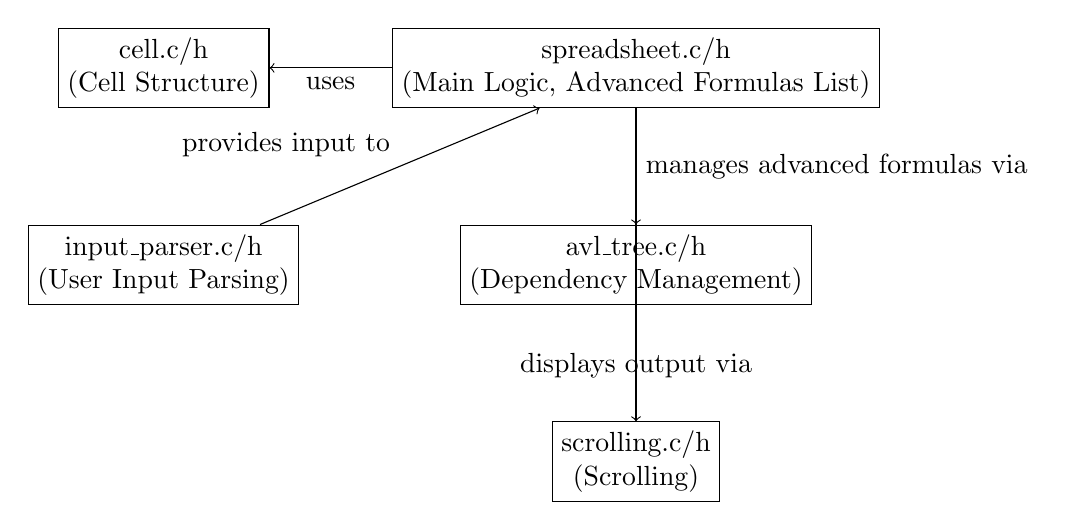
\begin{tikzpicture}[node distance=2.5cm, auto]
    % Nodes
    \node [draw, rectangle, align=center] (cell) {cell.c/h\\(Cell Structure)};
    \node [draw, rectangle, align=center, right of=cell, node distance=6cm] (spreadsheet) {spreadsheet.c/h\\(Main Logic, Advanced Formulas List)};
    \node [draw, rectangle, align=center, below of=spreadsheet] (avl) {avl\_tree.c/h\\(Dependency Management)};
    \node [draw, rectangle, align=center, below of=cell] (parser) {input\_parser.c/h\\(User Input Parsing)};
    \node [draw, rectangle, align=center, below of=avl] (scroll) {scrolling.c/h\\(Scrolling)};
    % Arrows
    \draw[->] (spreadsheet) -- node {uses} (cell);
    \draw[->] (spreadsheet) -- node {manages advanced formulas via} (avl);
    \draw[->] (parser) -- node {provides input to} (spreadsheet);
    \draw[->] (spreadsheet) -- node [below=1cm] {displays output via} (scroll);

\end{tikzpicture}
\caption{Software Architecture Diagram}
\label{fig:architecture}
\end{figure}

\section{Error Scenarios and Edge Cases}
The system handles several error and edge-case scenarios:
\begin{itemize}[noitemsep]
    \item \textbf{Cyclic Dependencies:} DFS and BFS routines detect cycles and prevent operations that would create them.
    \item \textbf{Division by Zero:} Cells performing division by zero are marked with an error.
    \item \textbf{Invalid Input Formats:} The parser in \texttt{handleOperation()} validates commands and flags malformed inputs.
    \item \textbf{SLEEP Function:} A negative value passed to the SLEEP function results in the cell storing the negative value while executing no delay (display time is set to 0.0).
    \item \textbf{Direct Assignment:} When a constant is assigned to a cell (e.g., \texttt{A1=2}), any stale dependency pointers are cleared so that previous errors are removed.
\end{itemize}

\section{Testing Strategy}
\begin{itemize}[noitemsep]
    \item Our testing strategy relied on a comprehensive test suite that generated a large number of commands to verify the correct recalculation and cycle detection.
    \item The output of the spreadsheet was compared with expected values to ensure accuracy.
\end{itemize}

\section{Demo and Repository Links}
\begin{itemize}[noitemsep]
    \item \textbf{Video Demo:} \url{https://yourvideodemo.link}
    \item \textbf{GitHub Repository:} \url{https://github.com/mayankgoel2005/lab1_2023CS10204_2023CS10186_2023CS10076}
\end{itemize}

\section{Conclusion}
The spreadsheet application is designed to handle both simple and advanced formulas efficiently. By maintaining a dedicated advanced formulas list, the program avoids the overhead of storing every cell in a range as a dependency. The design, supported by AVL trees for dependency management and a robust recalculation mechanism based on topological sorting, ensures that even complex dependency chains are updated correctly. This document has detailed the structure of the program, key functions, and error-handling strategies.

\end{document}
